\documentclass[aps, pra, 10pt, twocolumn, superscriptaddress,floatfix]{revtex4-1}

\usepackage{amsmath,amssymb,amsfonts}
\usepackage{braket}
\usepackage[breaklinks=true,colorlinks,citecolor=blue,linkcolor=blue,urlcolor=blue]{hyperref}
\usepackage{mathtools}
\usepackage{dsfont}

%%
\def \id {\mathds{1}}
\def \abs {\text{Abs}}
\newcommand{\norm}[1]{\lVert#1\rVert}
\DeclareMathOperator{\tr}{Tr}
\newcommand{\round}[1]{\ensuremath{\lfloor#1\rceil}}
\newcommand{\mi}{\mathrm{i}} %% roman "i"
%

\begin{abstract}
	In this notes we consider an estimation process of a rotation angle in an optical setup with unknown visibilities performed with both an online and an offline procedure.
\end{abstract}


\begin{document}
%
\title{Rotation angle estimation with unknown visibilities: online vs. offline procedure} 
%

\author{Federico Belliardo}
\email{federico.belliardo@sns.it}
\affiliation{NEST, Scuola Normale Superiore, I-56126 Pisa,~Italy}

\maketitle


\section{Introduction}
%
The previous work on optical quantum metrology has showed the possibility of reaching quantum enhanced scaling in the measurement of a rotation angle with the use of q-plates~\cite{Cimini2021}. In~\cite{Roccia2018} a Bayesian procedure to simultaneously measure the phase and the visibility in an optical setup has ben presented. In this work we want to somehow combine this two results and therefore perform a phase estimation measure in an optical setup with unknown visibility and simultaneously reach a quantum enhanced scaling. We are going to employ the q-plate setup of~\cite{Cimini2021}, see Fig.~\ref{fig:apparatus}, with three q-plates. This means the apparatus will be characterized by four visibilities: one for the configuration without active q-plates and three for the three configurations with only one q-plate active each. 
%
\begin{figure}[!t]
	\begin{center}
		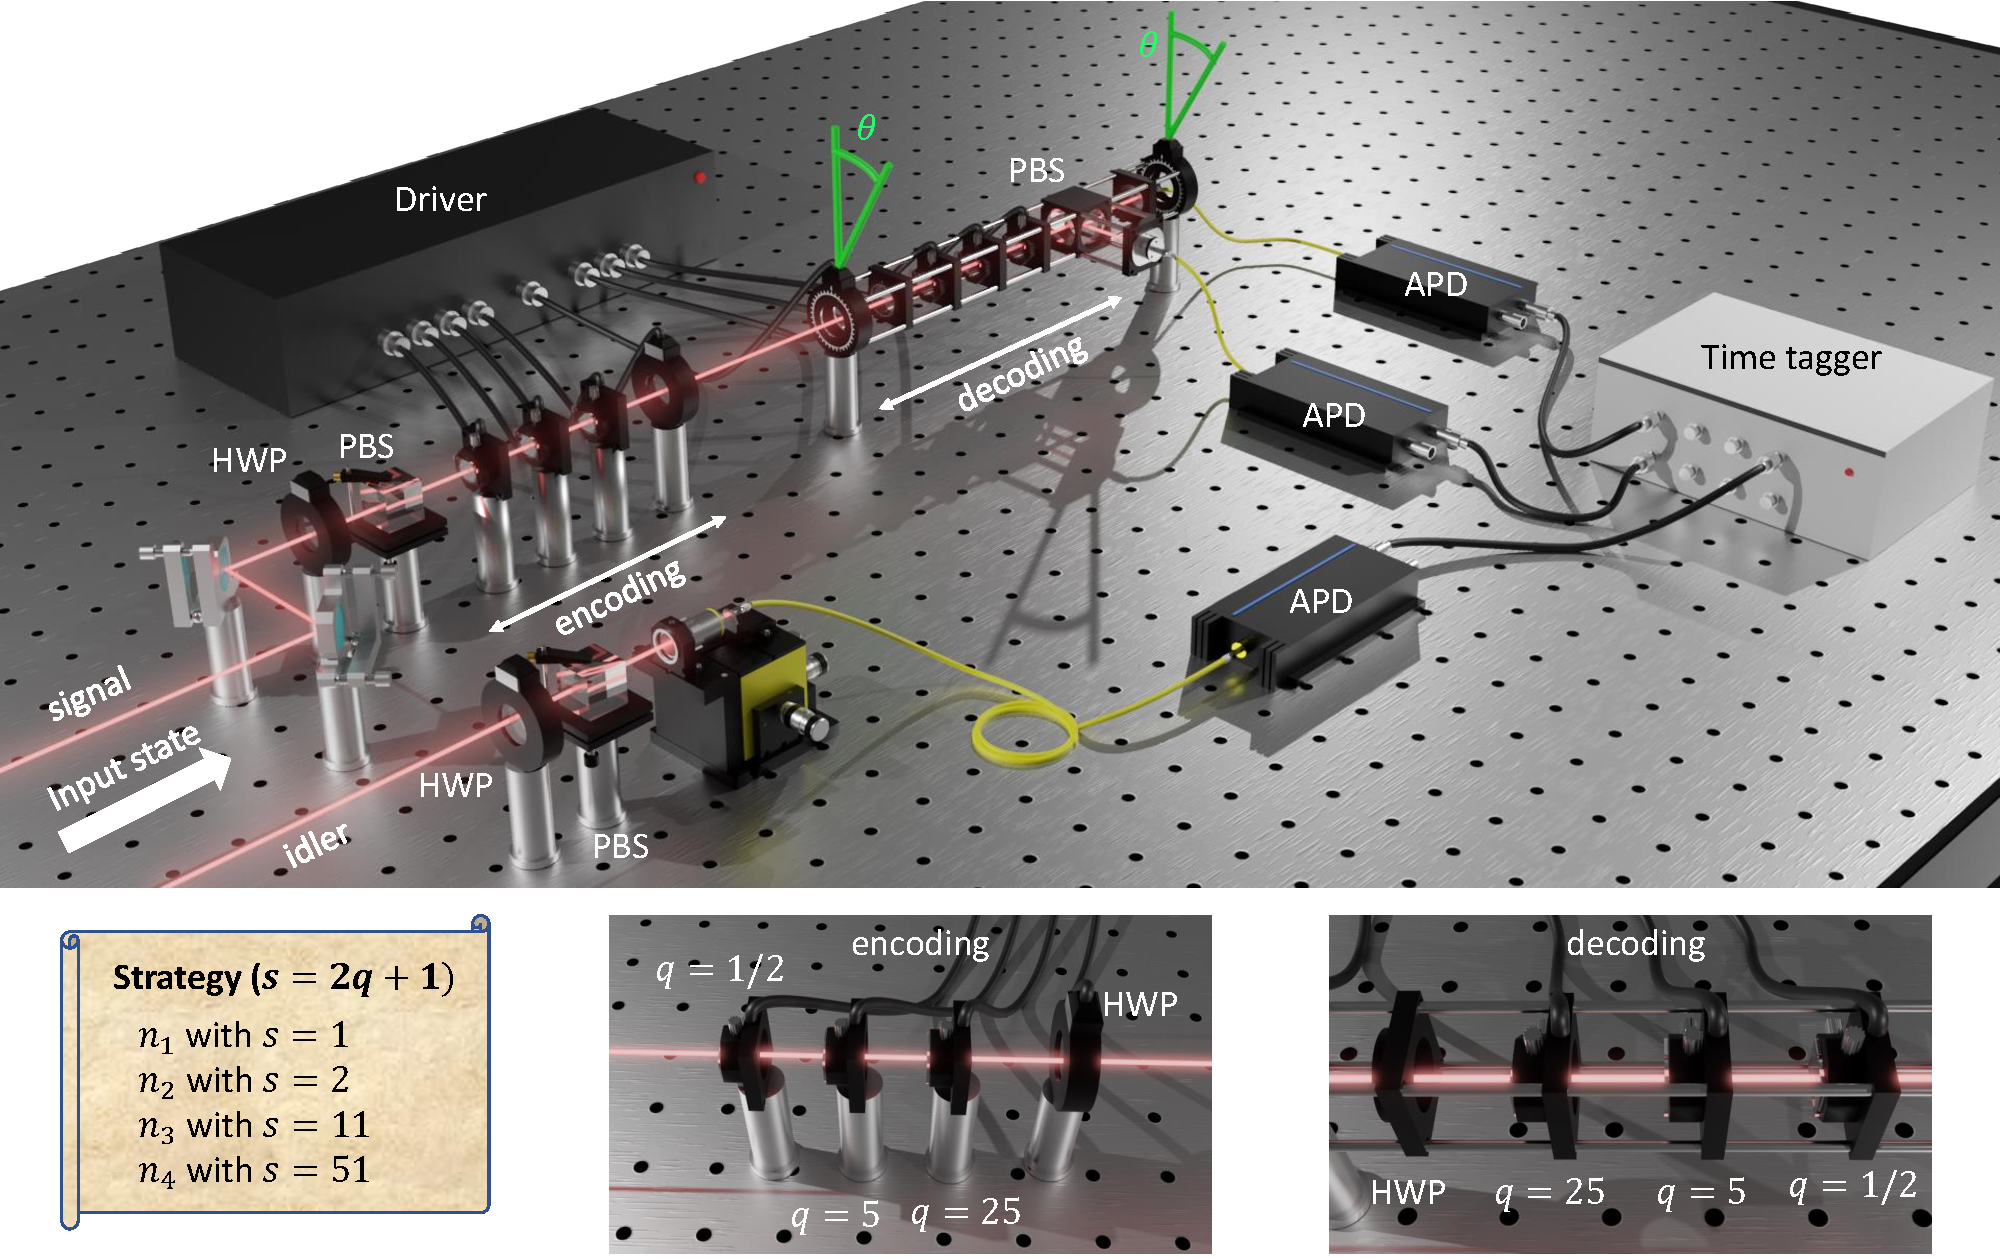
\includegraphics[width=0.5\textwidth]{FigureSetup.pdf}
	\end{center}
	\caption{View of the experimental apparatus with the three q-plates.}
	\label{fig:apparatus}
\end{figure}
%
We will suppose to have prior knowledge of the visibilities, that means, we suppose to know the distributions $\mathcal{P}_i (V_i)$ from which the four visibilities $V_0, V_1, V_2, V_3$ are extracted, without knowing the actual values of the visibilities in the particular experimental realization we are considering. In~\cite{Cimini2021} we presented an iterative offline method for the estimation of a phase with knowledge of the visibilities. Offline means that the number of photon measurements to be performed with each active q-plate is selected before the measurements are done and isn't changed during the experiment. Such offline procedure can't correct itself based on the outcome of the measurement but can be instructed to take into account the prior on the visibilities. The second approach we consider is the fully Bayesian procedure developed by Granade~\cite{Granade2012}. This method selects the next measurements to be done (the next q-plate) according to the posterior probability distribution for the unknown phase and visibilities.

\section{Offline procedure}
%
In order to determine the resource distribution to be used in the offline procedure we need the probability distribution for the outcomes of the two types of polarization measurements we are performing on the photons~\cite{Cimini2021, Belliardo2020}. Precisely in this probability distributions we can take into account the fluctuating visibilities. In our model the visibility of a q-plate is a stochastic variable $V$ extracted from a distribution $\mathcal{P} (V)$. Then the probability for the outcome $0$ of a Type-$0$ polarization measurement on a photon~\cite{Belliardo2020} is
%
\begin{equation}
	p_0 = \int dV p_0^V \mathcal{P} (V) \; ,
	\label{eq:defip0}
\end{equation}
%
where 
%
\begin{equation}
	p_0^V = \frac{1+V \cos(s \theta)}{2} \; .
	\label{eq:prob}
\end{equation}
%
Substituting Eq.~\eqref{eq:prob} in Eq.~\eqref{eq:defip0} we get
%
\begin{equation}
	p_0 = \int dV \frac{1+V \cos(s \theta)}{2} \mathcal{P} (V) \;  = \frac{1 + \mu_V \cos(s \theta)}{2} \; .
	\label{eq:der}
\end{equation}
%
where $\mu_V$ is the mean visibility. Therefore if the visibilities are fluctuating variables, only the their mean value is necessary to compute the resource distribution~\cite{Cimini2021}. 
%Similarly in a Bayesian approach we only need to learn the mean visibilities, that are encoded in the outcome distribution in Eq.~\eqref{eq:der} with the same form of regular visibilities. When performing an estimation with known (unknown) visibilities $V_1, V_2, V_3, V_4$ we can indifferently say that these are (we are learning) the actual visibilities or that these are (we are learning) the mean values of the visibility distributions. 
Three significant priors $\mathcal{P}_i(V_i)$ we might want to consider for the visibilities are reported in Fig.~\ref{fig:prior}.
%
\begin{figure}[!t]
	\begin{center}
		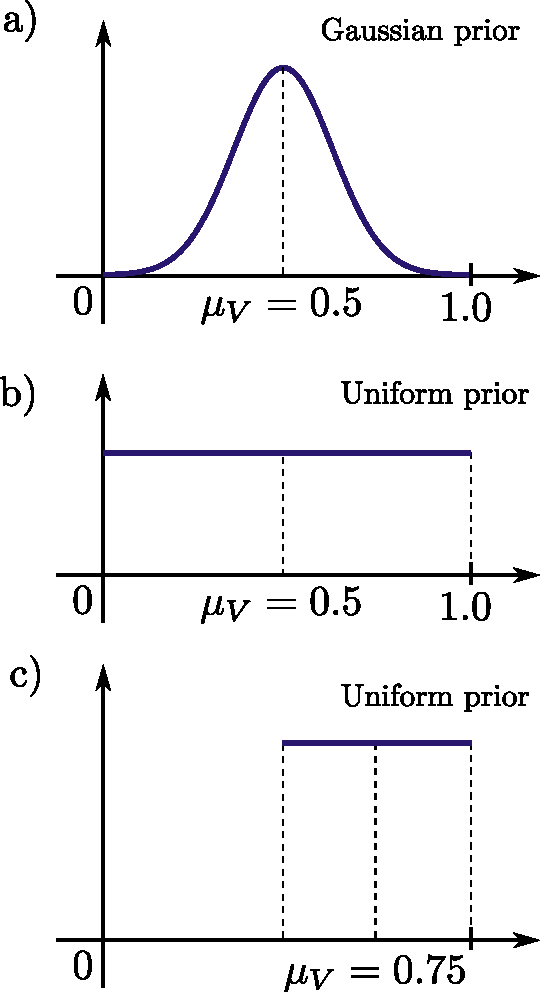
\includegraphics[width=0.3\textwidth]{priorProbability.pdf}
	\end{center}
	\caption{Possible prior probability distributions for the visibilities. For the iterative algorithm only the first moment (the mean) is important.}
	\label{fig:prior}
\end{figure}
%
The simulation has been done choosing a selection of values for $N$, that is meant to cover approximately uniformly the x-axis $N$ from $N=0$ to $N=3 \cdot 10^4$ in logarithmic scale. For each of the chosen $N$ the iterative algorithm has been applied $n = 100$ times. For each angle $\theta_j$, indexed with $j=1, \dots, J$ the error has been computed as
%
\begin{equation}
	\Delta \hat{\theta}_j = \sqrt{\frac{1}{n} \sum \limits_{k=1}^{n} | \hat{\theta}_{jk} - \theta_j |^2} \; ,
\end{equation}
%
and the error on this RMSE is
%
\begin{equation}
	\delta \Delta \hat{\theta}_j = \frac{\sigma \left( | \hat{\theta}_j - \theta_j |^2 \right)}{2 \sqrt{\sum \limits_{k=1}^{n} |\hat{\theta}_{jk} - \theta_j |^2}} \; ,
\end{equation}
%
with 
%
\begin{equation}
	\sigma \left( | \hat{\theta}_j - \theta_j |^2 \right) := \sqrt{\frac{\sum \limits_{k=1}^{n} | \hat{\theta}_{jk} - \theta_j |^4}{n} - \left( \frac{\sum \limits_{k=1}^{n} | \hat{\theta}_{jk} - \theta_j |^2 }{n} \right)^2} \; .
\end{equation}
%
In the plot we visualize the mean RMSE for the $J=17$ angles, i.e.
%
\begin{equation}
	\overline{\Delta \hat{\theta}} = \frac{1}{J} \sum \limits_{j=1}^{J} \Delta \hat{\theta}_j \; .
\end{equation}
%
The error (square root of the variance) of this mean will be
%
\begin{equation}
	\delta \overline{\Delta \hat{\theta}} = \frac{1}{J} \sqrt{\sum \limits_{j=1}^{J} (\delta \Delta \hat{\theta}_j)^2} \; .
	\label{eq:errory}
\end{equation}
%

\section{Online procedure}
%
In this section we apply the Bayesian algorithm presented by Granade~\cite{Granade2012} to our q-plates setup, with a few corrections due to the circular nature of the angular variable that we are going to measure. In every simulated experiment  a constant number of particles equal to $n_p = 1000$ has been used. The parameters to estimate are collected in the vector $\boldsymbol{x} := \left( \theta, V_1, V_2, V_3, V_4 \right)$, that contains the phase in the first entry and the four visibilities in the other ones. Being the Granade's method based on a particle filter, it represents internally the posterior probability distribution with the ensemble $\mathcal{E} := \lbrace \boldsymbol{x}^i, w^i \rbrace$, where $\boldsymbol{x}^i$ is the position of the $i$-th particle and $w^i$ its weight. The $j$-th component of the $i$-th particle of the ensemble will be represented as $x_j^i$, and could correspond to the phase if $j=0$, that is $x^i_0 = \theta^i$ or to one of the visibilities if $j=1, 2, 3, 4$, that is $x^i_j = V^i_j$. The mean of the angular values is computed as
%
\begin{equation}
	\hat{\mu}_0 := \arg \left[ \sum_{i=1}^{n_{p}} w^i \exp \left( \mi \theta^i \right) \right] \; ,
\end{equation}
%
while the mean values of the visibilities are
%
\begin{equation}
	\hat{\mu}_j = \sum_{i=1}^{n_p} w^i V^i_j \; .
\end{equation}
%
Together they form the vectorial mean of the distribution $\boldsymbol{\hat{\mu}} = (\hat{\mu}_0, \hat{\mu}_1, \hat{\mu}_2, \hat{\mu}_3, \hat{\mu}_4)$. The covariance matrix is defined as
%
\begin{equation}
	\text{Cov}_{ij} := \sum_{k=1}^{n_{p}} w^k (x^k_i - \hat{\mu}_i)  (x^k_j - \hat{\mu}_j) \; .
\end{equation}
%
If $i=1$ or $j=1$ then difference in $x^k_i - \hat{\mu}_i$ or $x^k_j - \hat{\mu}_j$ is actually the circular distance
%
\begin{equation}
	d(x^k_i, \hat{\mu}_i) = \pi - | (x^k_i - \hat{\mu}_i) \mod 2 \pi - \pi| \; .
\end{equation}
%
In the utility function we have considered only the variance of the phase, that is the component $\text{Cov}_{11}$ of the covariance matrix, so that the visibilities are treated as \textbf{nuisance parameters}. The resampling strategy of the Granade procedure has also undergone minor changes to adapt it to the phase estimation problem. We have simulated both algorithms (we didn't use the actual experimental data collected) with visibilities $V_1 = 0.900$, $V_2 = 0.875$, $V_3 = 0.850$ and $V_4 = 0.765$. The error of both the Bayesian and iterative algorithm is the mean error of the $17$ angles chosen in $[0, \pi)$ that have been measured in the actual experiment (maybe I should have simulated twice these angles). We propagate the errors in the Bayesian procedure in the same way they were propagated for the iterative procedure in the previous section. At difference with the offline algorithm we can't perform an estimation with a fixed number $N$ of total used resources, because the number of photons to use for each q-plate is a stochastic variable, that makes $N$ a stochastic variable also. Only the total number of used photons can be fixed. In order to find results that can be compared with the ones of the offline procedure we proceed as following. We repeat $n = 100$ times the Bayesian estimation for $N=30000$, and we save for each new photon measurement the estimator for $\theta$ and the total number of used resources up to that point. We associate all the estimations of $\theta$ made with a number of resources in the interval $[N, N + \Delta N]$, and apply to them the same analysis of the previous section, just as if they where coming from experiments with the same exact $N$. We associate the computed mean RMSE $\overline{\Delta \hat{\theta}}$ to the mean value of the total resources $N$. Each point of the plot will have not only an error bar on the $y$-axis given by Eq.~\eqref{eq:errory}, but also an error on the $x$-axis given by the dispersion of the $N$ values for the experiments that concurred in determining the given point on the plot. The value of $\Delta N$ changes according to $N$, in particular we have $\Delta N = 2$ for $N \in \left[2, 100 \right]$, $N = 20$ for $N \in \left[100, 1000 \right]$ and $\Delta N = 50$ for $N \in \left[1000, 30000 \right]$. In Fig.~\ref{fig:050vis} we report the simulation where the mean value of the visibilities for the prior of the offline procedure was $\mu_V = 0.50$.
%
\begin{figure}[!t]
	\begin{center}
		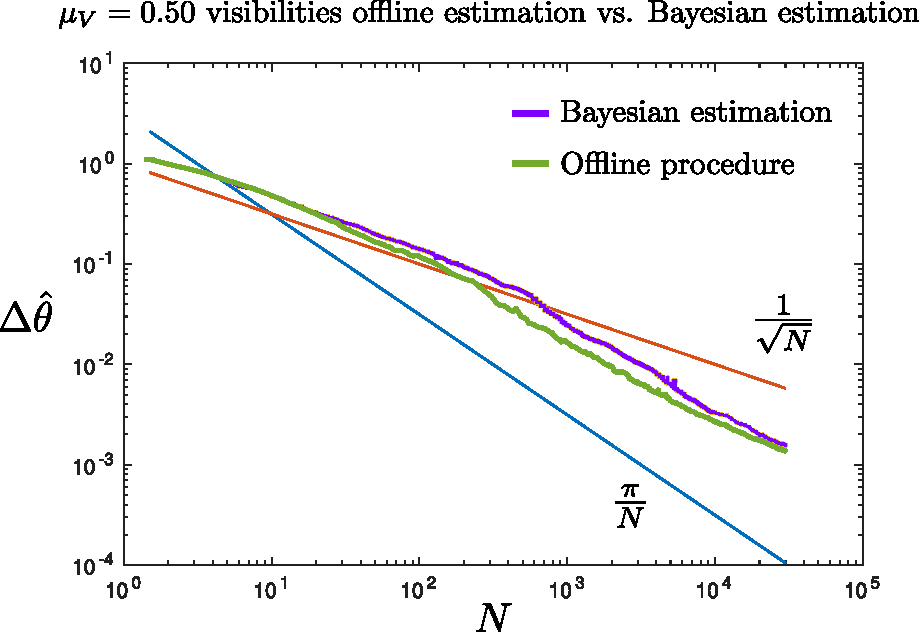
\includegraphics[width=0.5\textwidth]{050vis.pdf}
	\end{center}
	\caption{The violet line refers to the iterative estimation algorithm with a prior on the visibilities having $\mu_V = 0.50$ (it could be a Gaussian or a uniform prior). The green line is the Bayesian procedure with a uniform prior on the visibilities. The red and blue lines are respectively the standard quantum limit and the Heisenberg scaling scaling.}
	\label{fig:050vis}
\end{figure}
%
The two procedures (offline and online) differer in the region of enhanced scaling, and the Bayesian procedure is so efficient at extracting an approximate estimate of the visibilities, that no transient is apparently visible. In Fig.~\ref{fig:075vis} we report a simulation in which the prior distributions for the visibilities of the offline estimation have $\mu_V = 0.75$.
%
\begin{figure}[!t]
	\begin{center}
		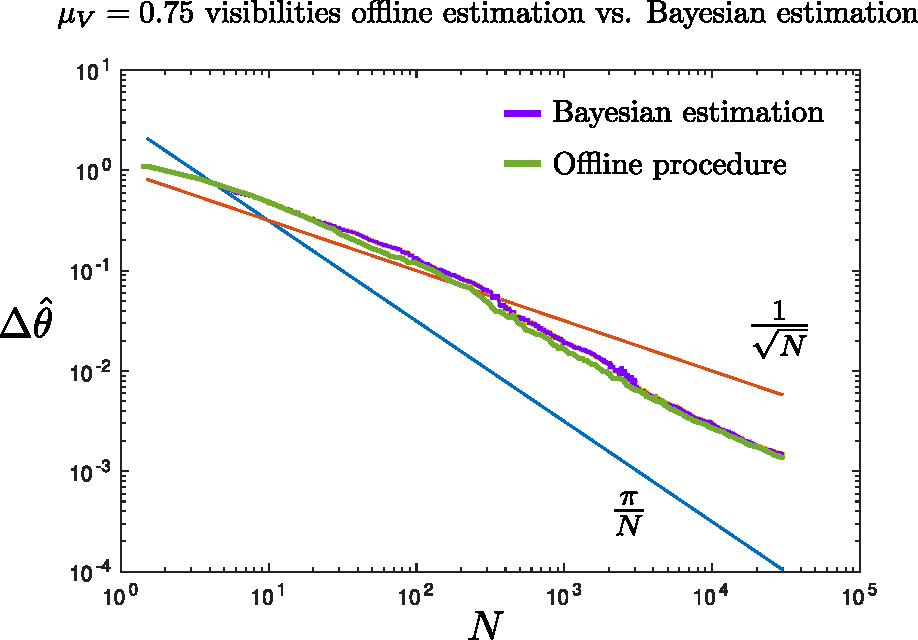
\includegraphics[width=0.5\textwidth]{075vis.pdf}
	\end{center}
	\caption{The violet line refers to the iterative estimation algorithm with a prior on the visibilities having $\mu_V = 0.75$. The green line is the Bayesian procedure with a uniform prior on the visibilities. The red and blue lines are respectively the standard quantum limit and the Heisenberg limit.}
	\label{fig:075vis}
\end{figure}
%
In all the Bayesian experiments performed so far the prior distributions on the visibilities are uniform in $[0, 1]$.
%
\begin{figure}[!t]
	\begin{center}
		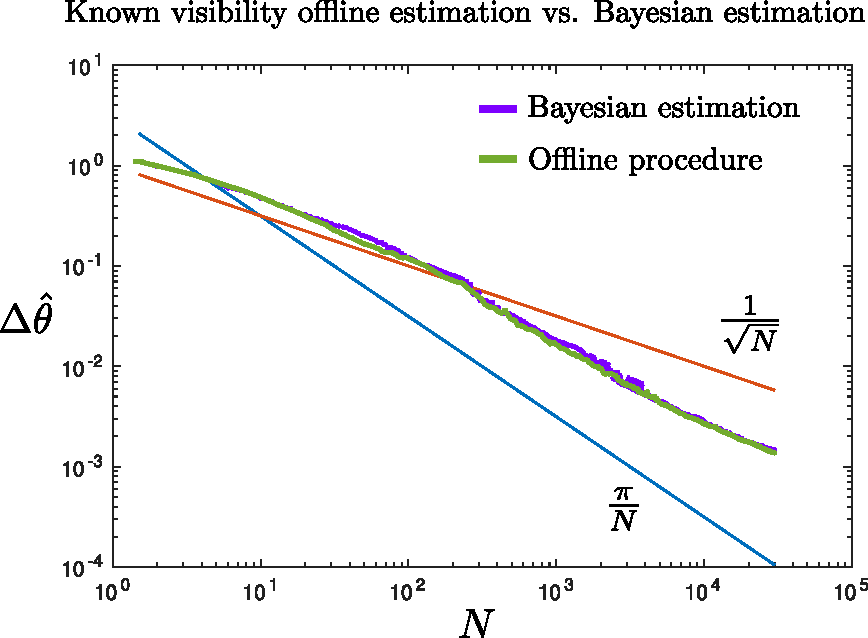
\includegraphics[width=0.5\textwidth]{trueVisibilities.pdf}
	\end{center}
	\caption{The violet line refers to the iterative estimation algorithm with perfect knowledge of the visibilities. The green line is the Bayesian procedure with a uniform prior on the visibilities. The red and blue lines are respectively the standard quantum limit and the Heisenberg limit.}
	\label{fig:trueVisibilities}
\end{figure}
%
In Fig.~\ref{fig:trueVisibilities} we compare an offline procedure with perfect knowledge of the visibilities, with an online procedure that has to learn them step by step. Here it becomes apparent how efficient is the Bayesian learning of the nuisance parameters. A very imprecise knowledge of the visibility is sufficient to find a good approximation of the optimal strategy. A more fair comparison would give also the Bayesian algorithm the exact visibilities from the start, so that it doesn't need to learn them. We gave the Bayesian algorithm a delta-like prior distribution concentrated on the correct visibilities, and the outcome was that of Fig.~\ref{fig:exactVisibilitiesBayesian}
%
\begin{figure}[!t]
	\begin{center}
		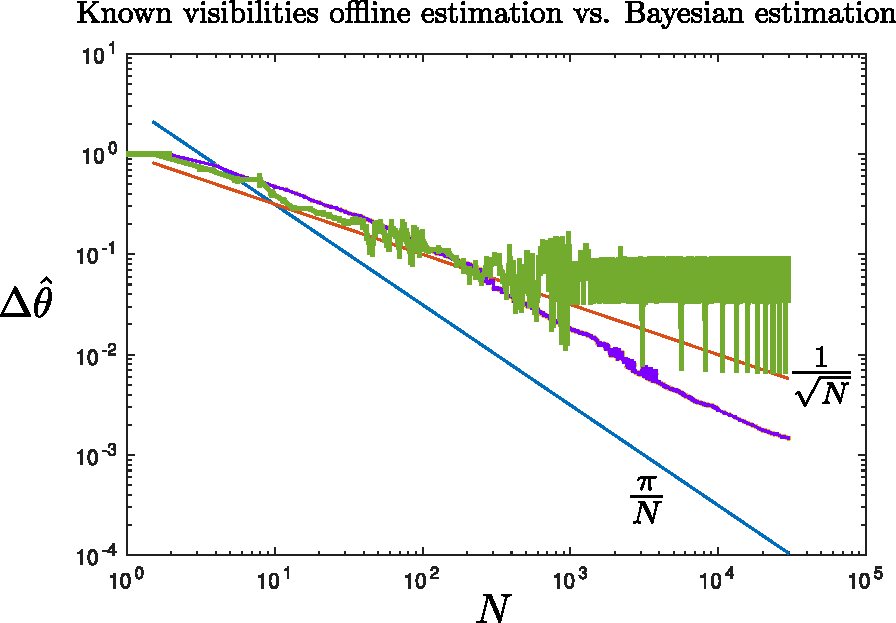
\includegraphics[width=0.5\textwidth]{exactVisibilitiesBayesian.pdf}
	\end{center}
	\caption{The violet line refers to the iterative estimation algorithm with perfect knowledge of the visibilities. The green line is the Bayesian procedure with a delta-like prior on the visibilities. The red and blue lines are respectively the standard quantum limit and the Heisenberg limit.}
	\label{fig:exactVisibilitiesBayesian}
\end{figure}
%
The estimation procedure fails because somehow the resampling procedure fails. We have tried to switch off the resampling and increase the number of particles to $n_{p} = 5000$, thus obtaining the results of Fig.~\ref{fig:krz}.
%
\begin{figure}[!t]
	\begin{center}
		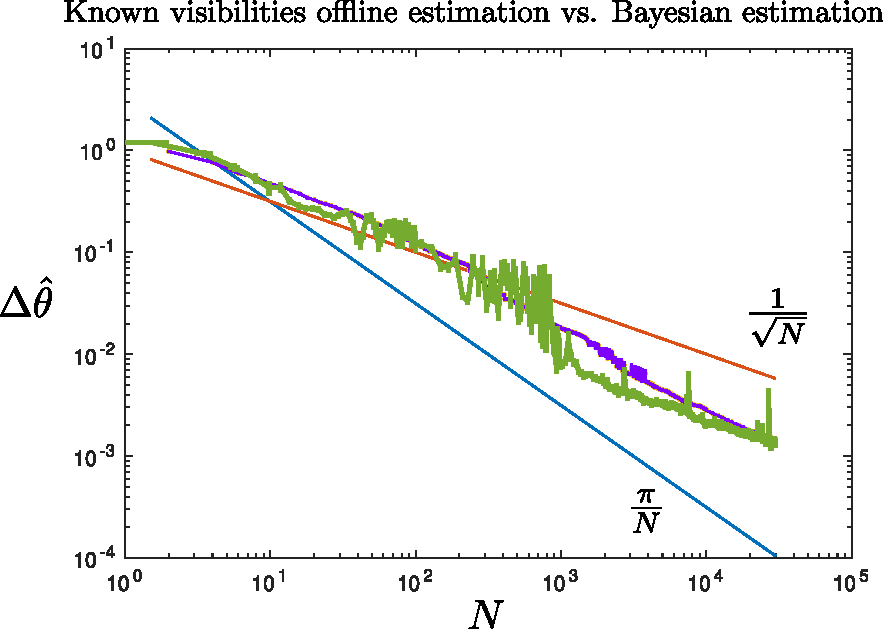
\includegraphics[width=0.5\textwidth]{bayesianNoResampling5000particles.pdf}
	\end{center}
	\caption{The violet line refers to the iterative estimation algorithm with perfect knowledge of the visibilities. The green line is the Bayesian procedure with a delta-like prior on the visibilities. In these experiments we have switched off the resampling and increased the number of particles to $n_p = 5000$. The red and blue lines are respectively the standard quantum limit and the Heisenberg scaling scaling.}
	\label{fig:krz}
\end{figure}
%
This last plot presents a completely failed estimation regime from $N=10$ to $N=1000$ and a somewhat more stable regime from $N = 1000$ to $N=30000$. For this last resource interval the Bayesian estimation seems to do better than the iterative one, although a few peaks in the error indicate that the resource distribution chosen by the Bayesian procedure might have been a little too hazardous. If we don't use the delta-like prior, but instead instruct the algorithm to perform the estimation of a single parameter, we obtain the same result of Fig.~\ref{fig:krz}.


\begin{thebibliography}{100}
			
	\bibitem{Cimini2021} V Cimini \textit{et al.}, \href{http://arxiv.org/abs/2110.02908}{arXiv:2110.02908 (2021).}
	%
	
	\bibitem{Roccia2018} E Roccia \textit{et al.}, \href{https://www.osapublishing.org/optica/abstract.cfm?uri=optica-5-10-1171}{Optica~{\bf 5}, 1171-1176 (2018).}
	%
		
	\bibitem{Belliardo2020} F Belliardo and V Giovannetti, \href{https://link.aps.org/doi/10.1103/PhysRevA.102.042613}{Phys. Rev. A~{\bf 102}, 042613}.
	%
	
	\bibitem{Granade2012} C E Granade \textit{et al.} 2012 \href{https://doi.org/10.1088/1367-2630/14/10/103013}{New J. Phys. {\bf 14} 103013}.
	%
	
\end{thebibliography}

\end{document}